\addchapheadtotoc
\chapter{Applied Radiation Model}\label{chapter:Example}
The complexity of the radiation solver resulting from both its theoretical foundation as well as its computational implementation calls for an extensive series of validation and performance studies.

Three test geometries are presented in this chapter for verification and profiling using the two methods discussed in section \ref{section:ModelForThisStudy}. The configurations include the canonical one-dimensional plane-parallel medium, a three-dimensional backwards-facing step combustor, and a three-dimensional Pratt \& Whitney NEO aeronautical combustor. 
These three test cases provide an excellent basis to verify the solution methods and test their performances. 



\section{One dimensional plane-parallel medium}
The plane-parallel medium provides a useful, one dimensional case to test the MCRT code. The geometry is shown in figure \ref{fig:PlaneParallelGeometry}.

The geometry consists of two parallel plates surrounding a radiatively-participating medium. The system is one-dimensional (implemented into OpenFOAM using either ray-reflections along the off-axis boundaries, or through a long stretch in both the Y and Z directions). The simulation is steady, and the walls are black-bodies (perfect absorbers and emitters).
Using this configuration, the user can artificially select an absorption coefficient, $\kappa{}$, medium temperature, $T$, and wall temperatures $T_w$.

Additionally, the relative simplicity of the configuration allows for reduced-complexity numerical solution described in appendix (IN APPENDIX OR PUT HERE?). 
This "analytical" solution can be used for verification of the solver under variable absorption coefficient, temperatures, and scattering coefficient (not included in this model).

The one-dimensional nature of the system also results in the least-ideal scaling for multi-node simulations. \textit{Provides useful understanding of how the runtime and memory usage scale for each solver under worst-case situations.}

\subsection{Results}
Figure \ref{fig:PP_kappatest} presents a comparison of the MCRT solutions alongside the analytical solutions. The configuration is tested under a variety of absorption coefficients, temperatures, and Monte-Carlo ray counts. The various case conditions are presented in table \ref{table:PPcomp}.

\begin{figure}
  \begin{subfigure}{1\textwidth}
  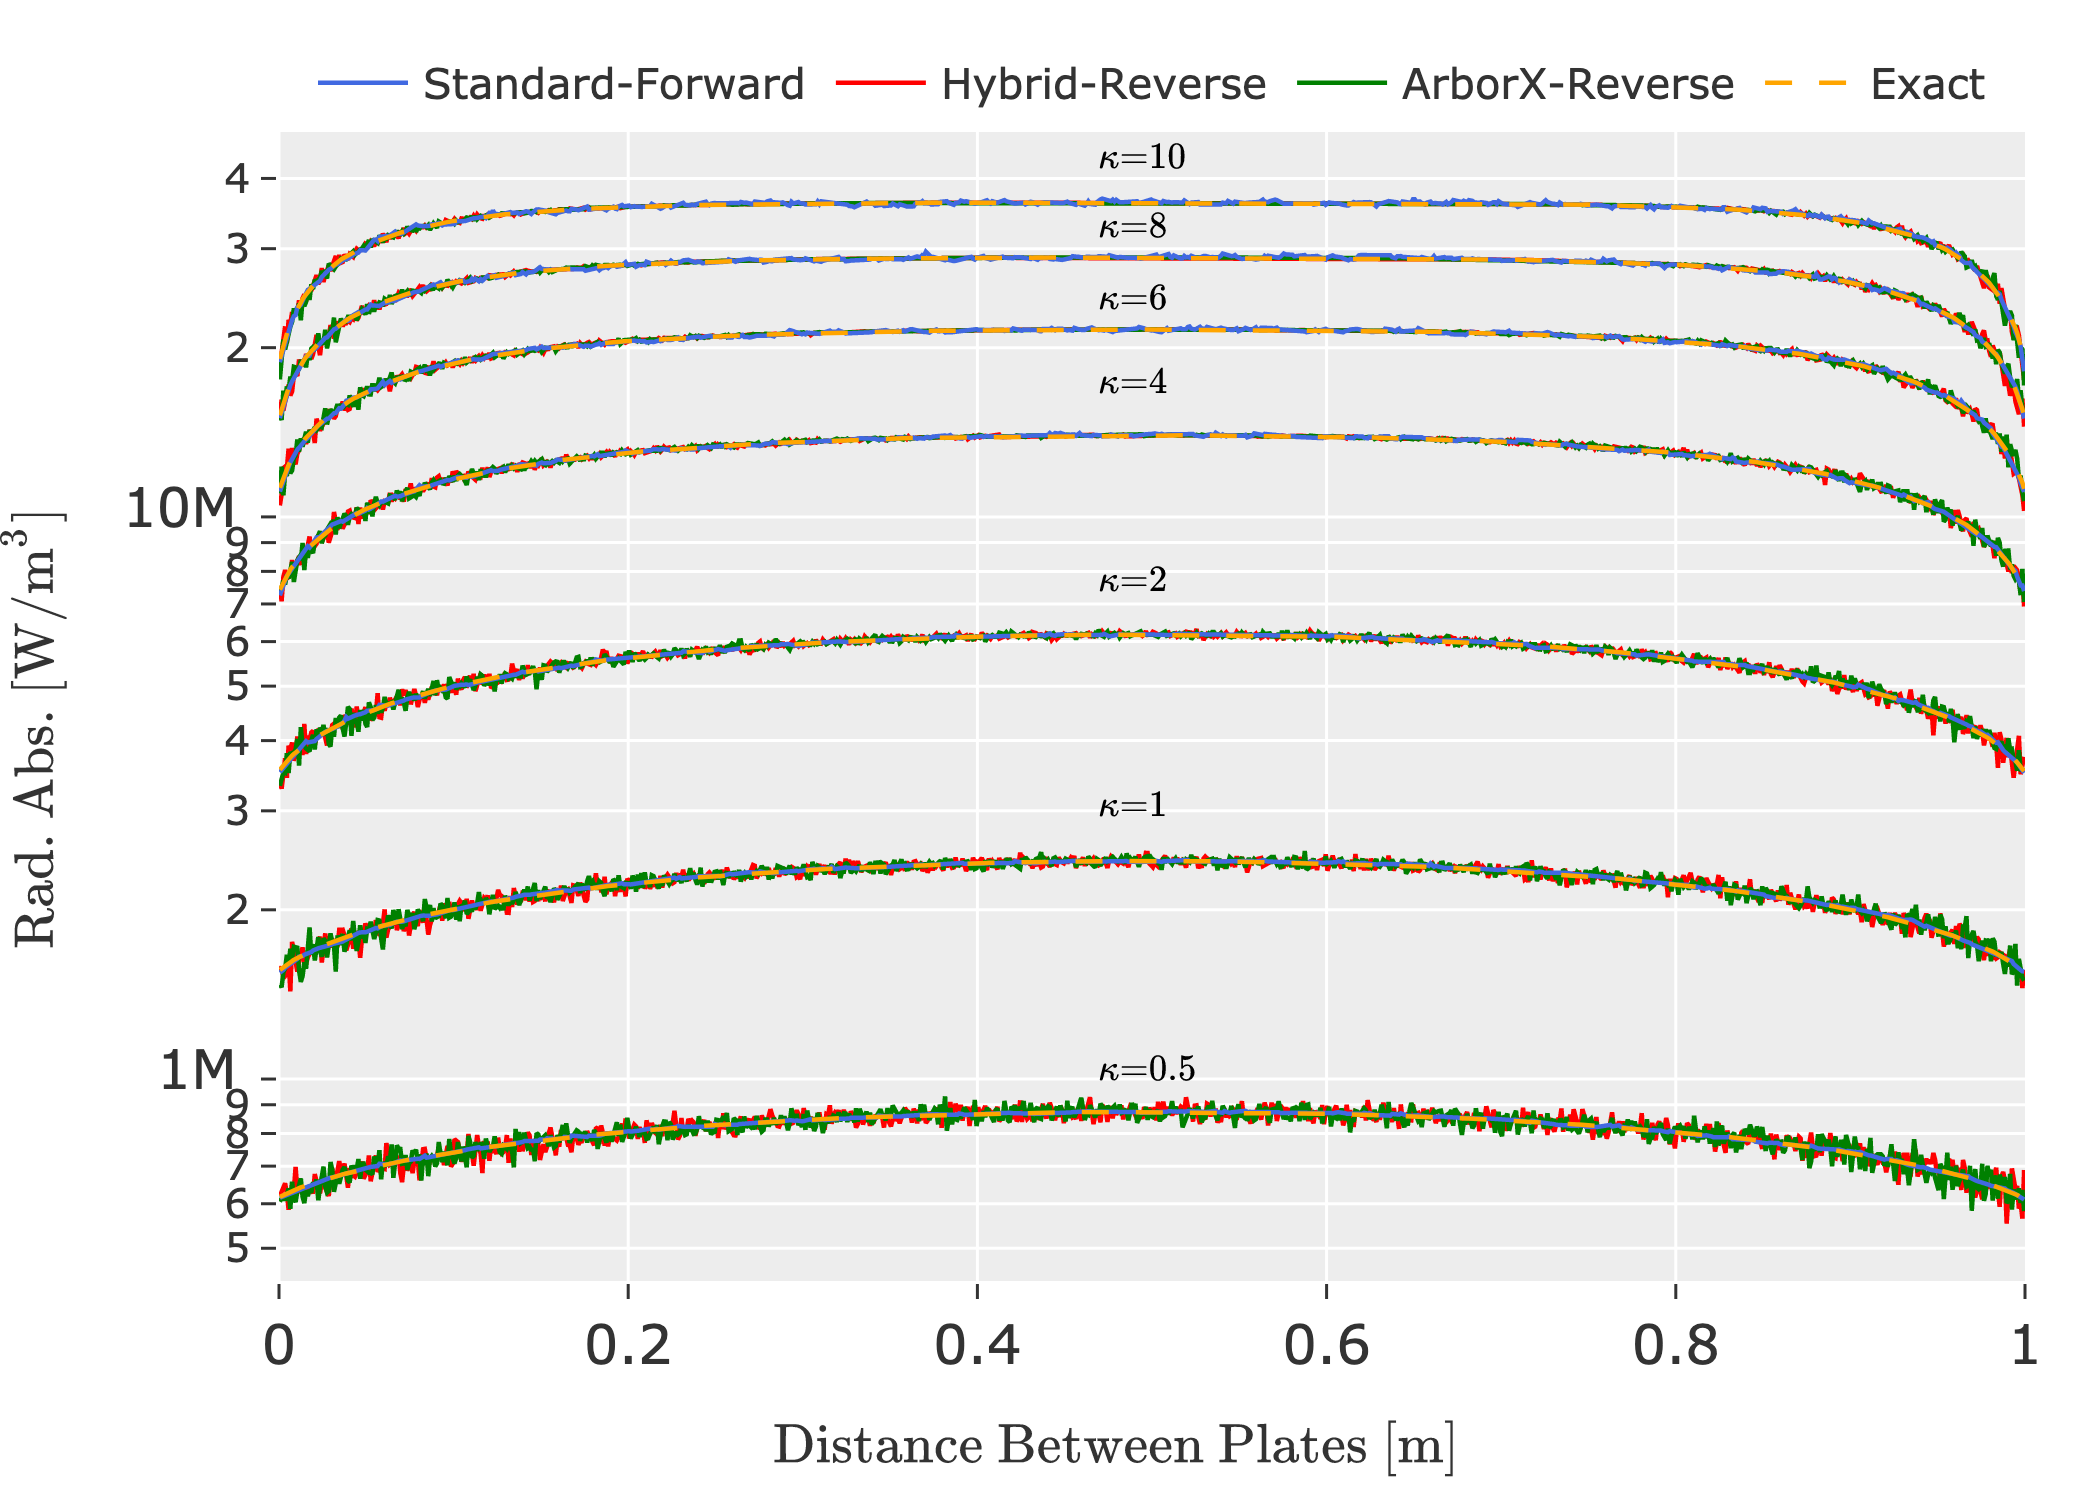
\includegraphics[width=\linewidth]{figures/ch4/PPcomparison1.png}
  \caption{Variable absorption coefficient with T=$2000$K, N$_r$=$1000$, N$_{cells}$=1000.}
  \label{fig:PPcomp_kappa}
  \end{subfigure}
  \begin{subfigure}{1\textwidth}
  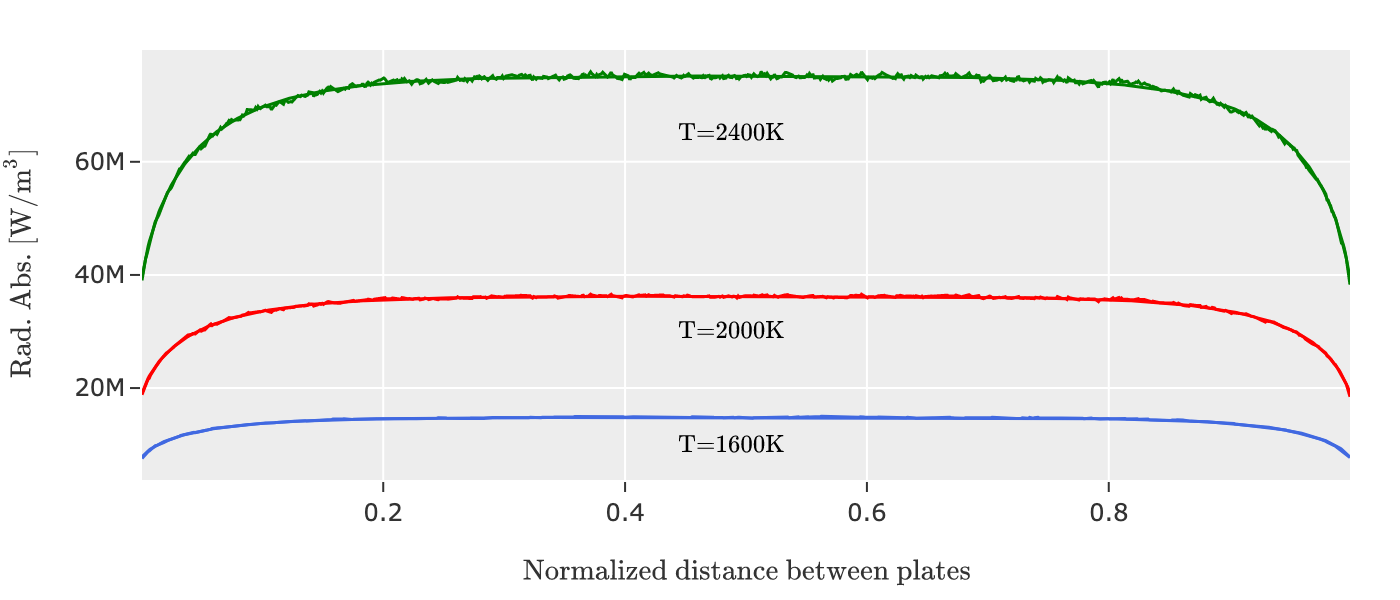
\includegraphics[width=\linewidth]{figures/ch4/PPcomparison2.png}
  \caption{Variable temperature with $\kappa{}$=$10$ m$^{-1}$, N$_r$=$1000$, N$_{cells}$=1000.}
  \label{fig:PPcomp_temp}
  \end{subfigure}
  \begin{subfigure}{1\textwidth}
  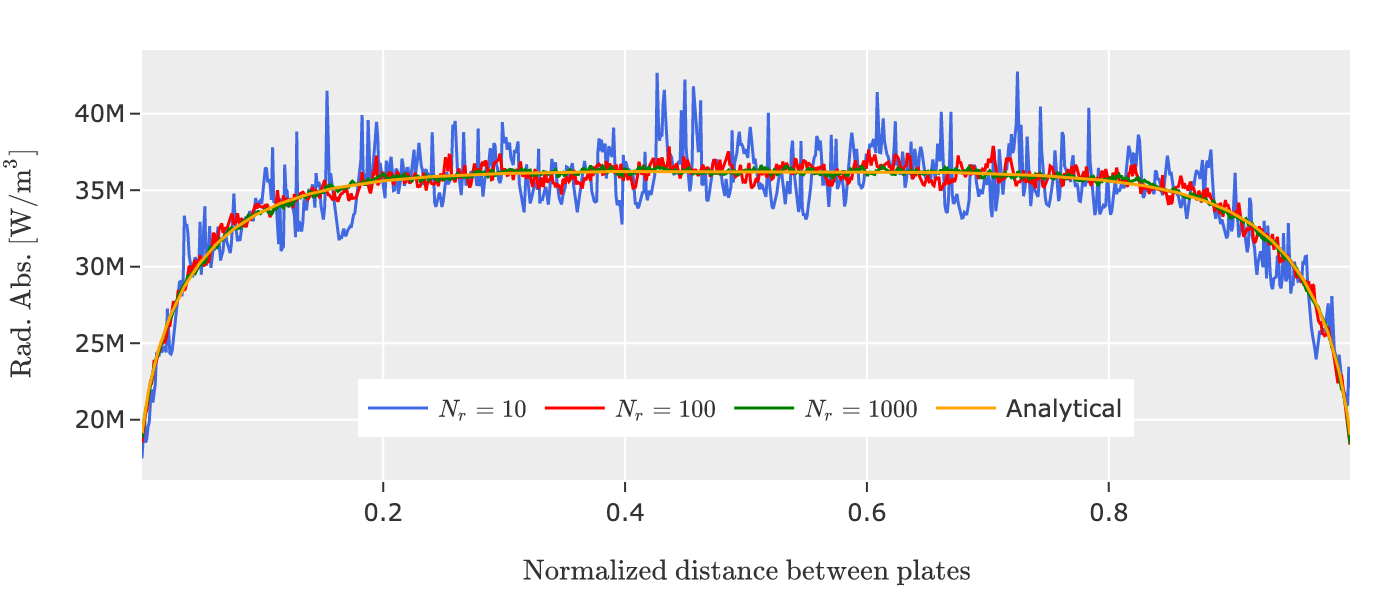
\includegraphics[width=\linewidth]{figures/ch4/PPcomparison3.png}
  \caption{Variable number of rays emitted per cell (N$_r$) with $\kappa{}$=$10$ m$^{-1}$, T=$2000$K, N$_{cells}$=1000.}
  \label{fig:PPcom_nrays}
  \end{subfigure}
  \label{fig:PPcomp}
\end{figure}

Results show excellent comparison between the MCRT and analytical implementations. 
The lower ray counts show a higher degree of variability resulting from the stochastic nature of the MCRT method. 
Increasing absorption coefficient leads in an increase of radiative emission and re-absorption, with re-absorption increasing at a higher rate resulting in a net increase of radiative source.

These expected results demonstrate the requirement for RTE modeling in optically thick media. Not only does radiative emission result in heat loss from computational cells, but also the re-absorption can be high enough to require modeling of the self-absorption process of radiation.

\subsection{Profiling}


\section{Backwards-Facing Step Combustor}
The backwards-facing step (BFS) combustor is a convenient geometry often used in the field of fluid dynamics for a simple, repeatable geometry to analyze turbulence, heat transfer and combustion.

\begin{figure}{1\textwidth}
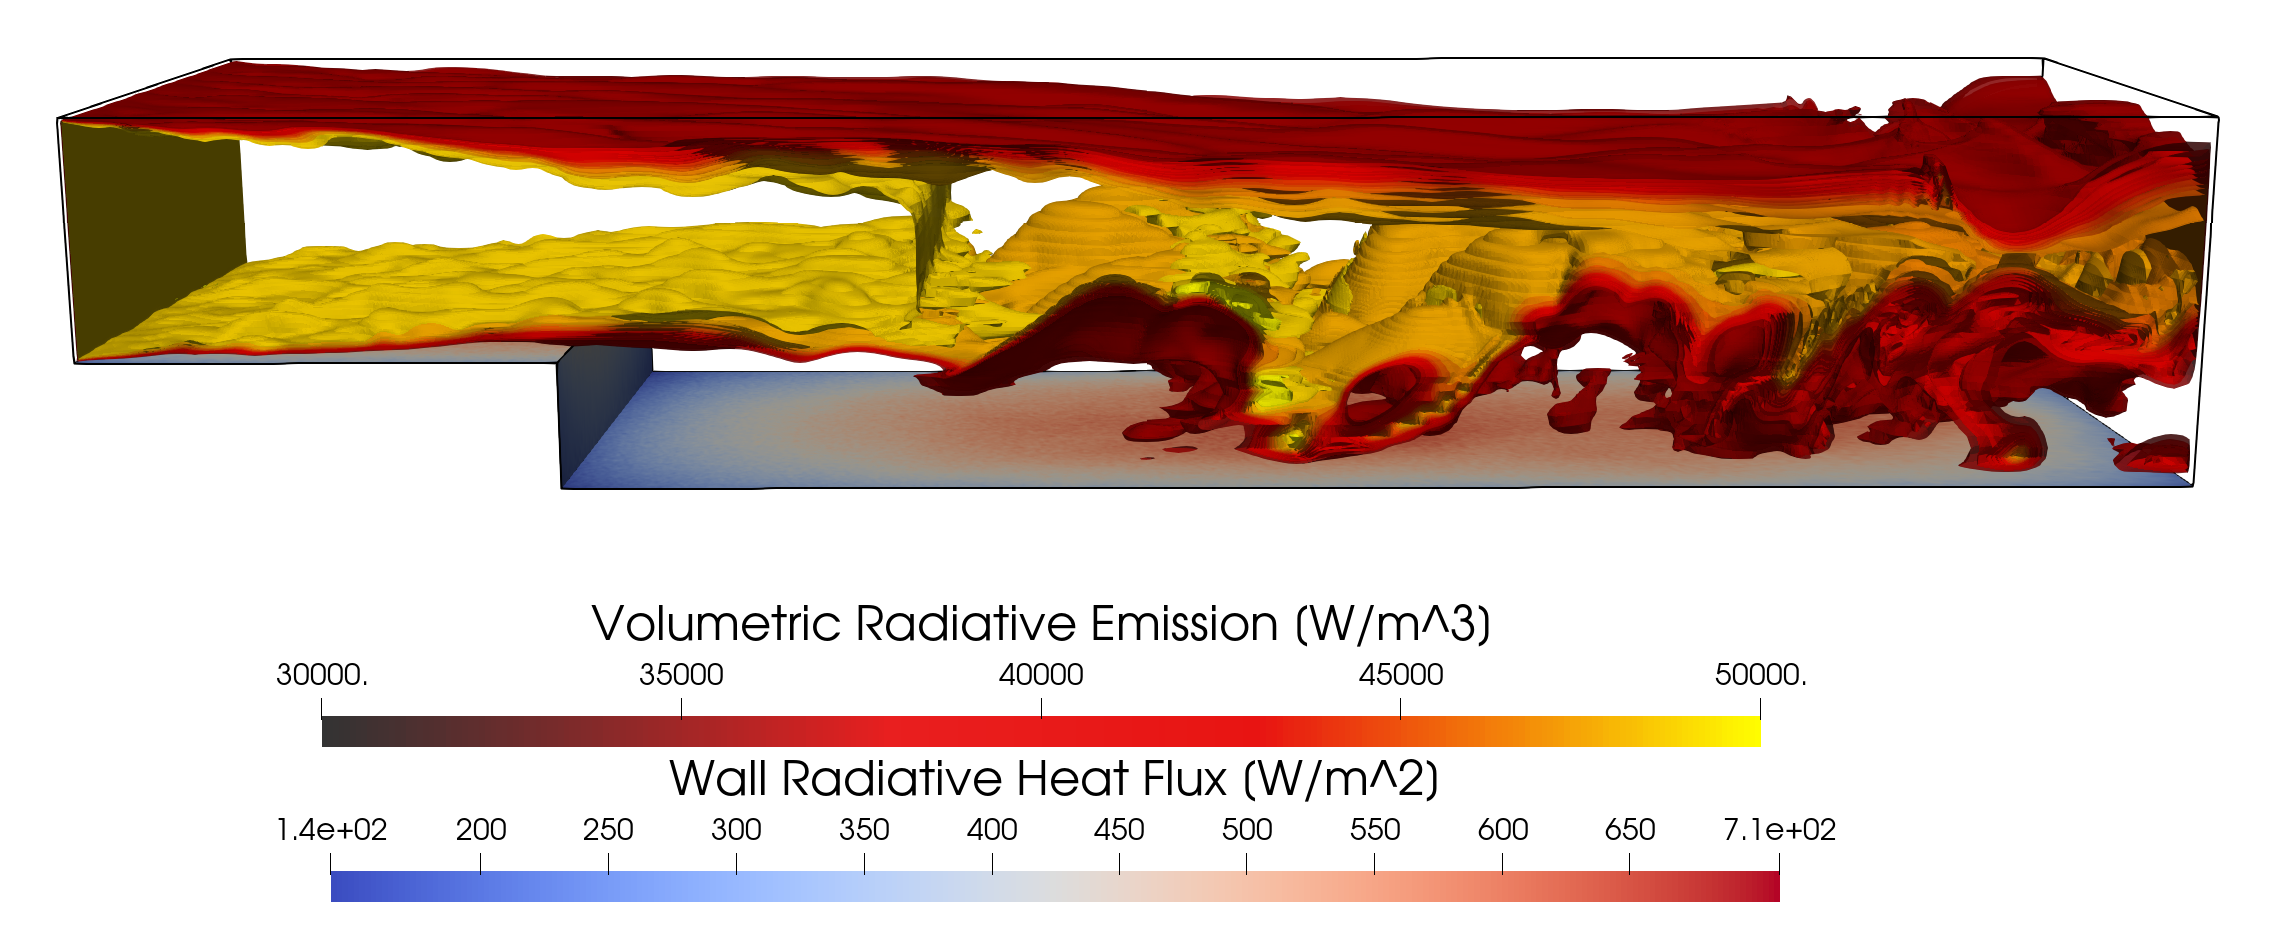
\includegraphics[width=\linewidth]{figures/ch4/BFS_volwallflux3.png}
\caption{Variable absorption coefficient with T=$2000$K, N$_r$=$1000$, N$_{cells}$=1000.}
\label{fig:BFS_geometry}
\end{figure}


\subsection{Background}
\subsection{Results}
\subsection{Model Performance}
\section{Pratt \& Whitney NEO Combustor or Pool Flame}
